\chapter{Models}
The first deep learning-based object detection models emerged after a breakthrough in ImageNet Large Scale Visual Recognition Challenge (ILSVRC) in 2012 when Alex Krizhevesky et al. proposed a deep and wide CNN classification model. The so-called AlexNet outperformed traditional state-of-the-art models.  This architecture was later exploited as a feature extractor for the CNN-based object detection model R-CNN, which also surpassed the previous best results on PASCAL VOC 2012. Since then, many CNN-based object detection models were introduced.

Generally, they can be categorized into two types: one-stage detectors and two-stage detectors. The latter approach consists of a regional proposal step, followed by classification and bounding box regression. This means that the model initially generates interesting regions, which are then analyzed one-by-one. In contrast, one-stage detectors are based on a global regression and classification, requiring a single pass through the network, and thus they are usually faster but less accurate. A common property of both approaches is that we can easily substitute the models' feature extractor. 

For our comparison, we have chosen three state-of-the-art models: Faster R-CNN, Cascade R-CNN, and RetinaNet. The first one was proposed in 2015, and it is a well-known example of two-stage detectors. The model is considered to be well-established as it has a reasonable accuracy/speed tradeoff and is easy to modify. In our work, Faster R-CNN serves as a baseline for our comparison. The next one, Cascade R-CNN, is an extension to Faster R-CNN, which improves the performance by addressing some of its caveats. Finally, RetinaNet is a recent one-stage detector introduced by the Facebook AI Research team (FAIR), aiming to match the two-stage detectors' accuracy while preserving one-stage detectors' speed. We describe all these models in detail in the following sections.

\section{Architecture}
The architecture of models can be divided into two parts: backbone and detection head. The backbone is responsible for computing feature maps from the input image. The feature maps are then used for predicting the bounding boxes and classifications by the detection head. All our models use ResNet as a backbone. Except for the Faster R-CNN's backbone, the ResNet is additionally extended with Feature Pyramid Network (FPN), which helps with detecting objects at different scales. We describe ResNet, FPN, and each model's detection head in the following sections.

\section{ResNet}
Deeper neural network architectures are harder to train because of the disappearing gradient. As the gradient is backpropagated through the network, the repeated multiplication by values between 0 and 1 makes the gradient very small, and eventually, it vanishes. Thus the earlier layers are not trained properly. This is called the vanishing gradient problem. 

ResNet is a CNN-based image recognition model proposed in 2015 to solve the difficulties of training deeper architectures by introducing skip connections between the layers allowing to train up to 1001-layer deep architectures. For comparison, the previous state-of-the-art model VGG consists of up to 19 sequentially stacked layers (see Figure \ref{fig:vgg_resnet}).

\begin{figure}[h]
    \centering
    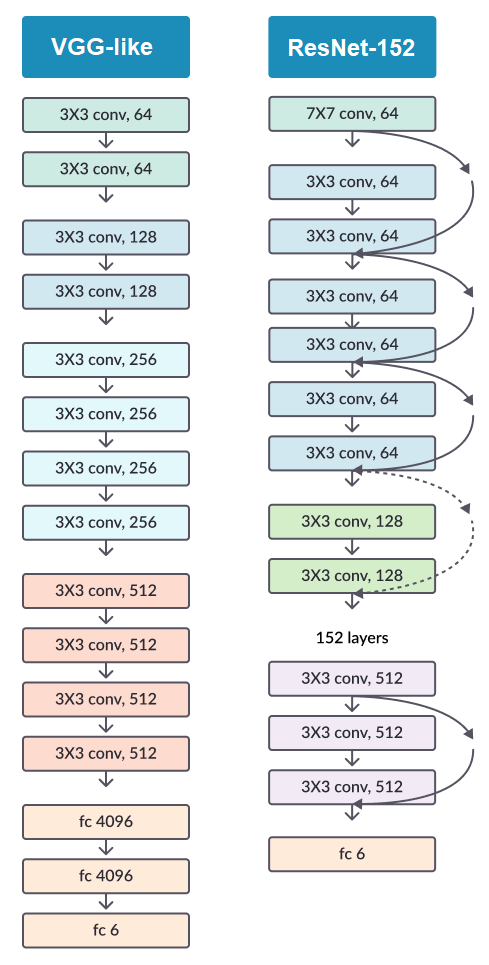
\includegraphics[width=0.4\linewidth]{Sources/Figures/vgg_resnet.png}
    \caption{A visual comparison of a VGG-like network and ResNet.}
    \label{fig:vgg_resnet}
\end{figure}

Skip connections are realized by performing identity mapping. Its outputs are then simply added to the outputs of the stacked layers (see Figure \ref{fig:residual_block}). This helps with propagating the gradient deeper in the network. 

\begin{figure}[h]
    \centering
    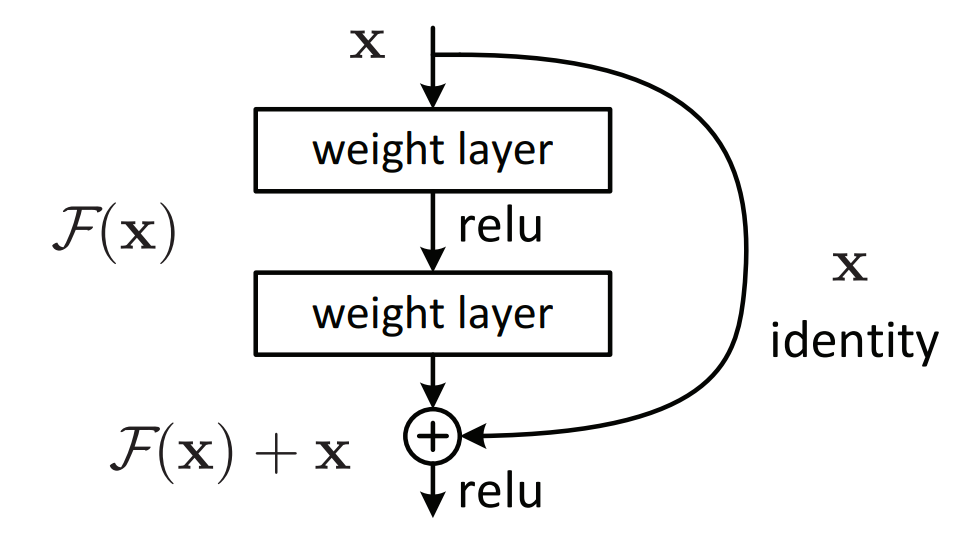
\includegraphics[width=0.4\linewidth]{Sources/Figures/residual_block.png}
    \caption{Visualization of a skip connection.}
    \label{fig:residual_block}
\end{figure}

\section{Feature Pyramid Network}
One of the challenges of object detectors is to detect objects at different scales. To approach this, we can simply process the same image at different scales. However, this naive method is very inefficient and requires a lot of computation time and memory. A more efficient way would be to take the computed feature maps of different scales and use them for the prediction. But the feature maps closer to the input are composed of low-level features (e.g., edges), which are not very valuable for accurate predictions. We can visualize these approaches as a pyramid of images or features (see Figure ). 

\begin{figure}[h]
    \centering
    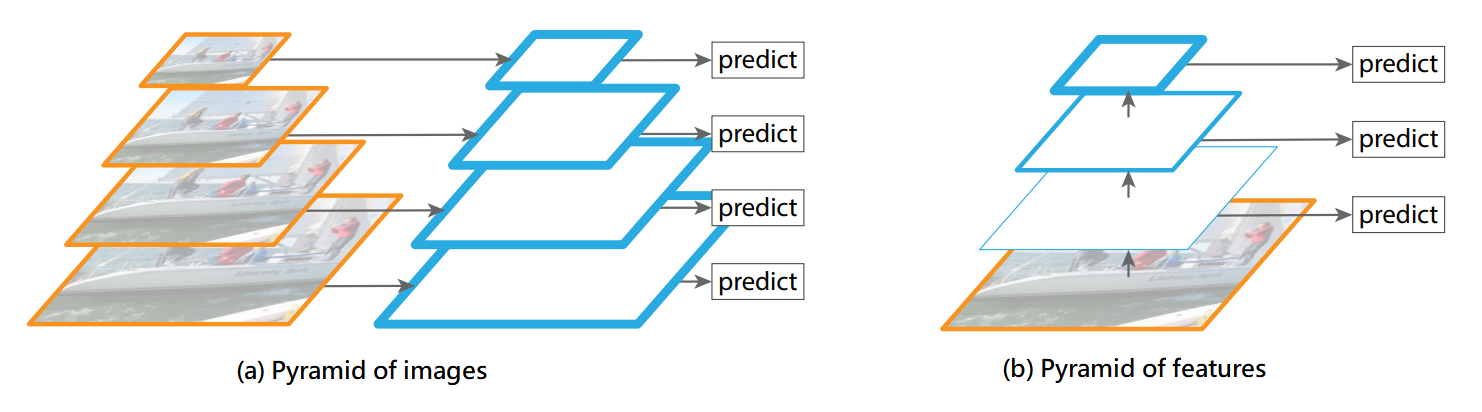
\includegraphics[width=\linewidth]{Sources/Figures/pyramids.png}
    \caption{(a) Features are computed independently for each scale; (b) exploits the computed feature maps of feature extractor. Adapted from \todo{cite}}
    \label{fig:pyramids}
\end{figure}

In 2017 Lin et al. proposed Feature Pyramid Network that enhances the feature maps from lower pyramid levels with high-level features. To achieve this, the construction of the feature pyramid involves a bottom-up pathway and a top-down pathway (see Figure \ref{fig:fpn}). The bottom-up pathway is the conventional CNN feature extractor, which gradually produces smaller and smaller feature maps, but with high-level features (we say that they are semantically richer). The top-down pathway upsamples the semantically richer features to match the higher resolution of the feature maps in the bottom-up pathway. These different feature maps are then added together via lateral connections between them. Those connections also help to make training easier, similarly as in ResNet.  Finally, these semantically enriched multi-scale feature maps can be used by the detection head of an object detection model. 

\begin{figure}[h]
    \centering
    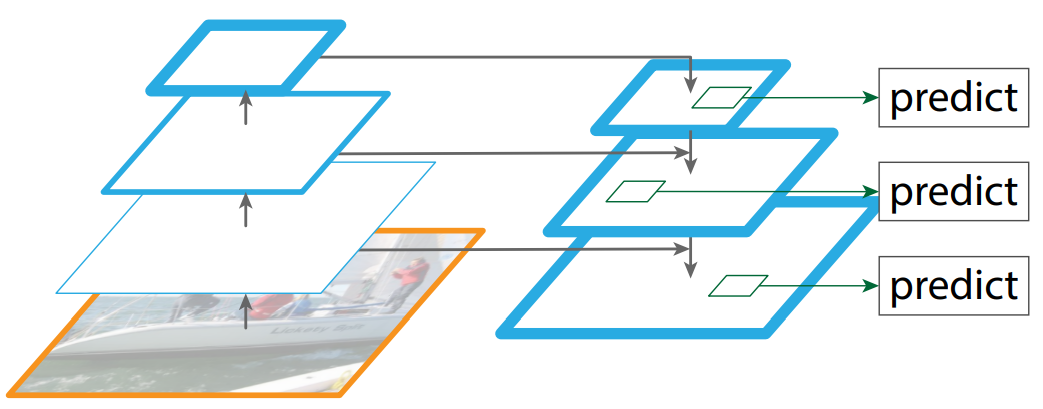
\includegraphics[width=0.6\linewidth]{Sources/Figures/fpn.png}
    \caption{FPN with bottom-up pathway (left), top-down pathway (right) and lateral connections (horizontal arrows).}
    \label{fig:fpn}
\end{figure}

\section{Faster R-CNN}
The first model we describe is Faster R-CNN proposed in 2015 by the same co-authors of ResNet. As we mentioned at the beginning of the chapter, Faster R-CNN is a two-stage detector. Firstly, it generates candidate regions of interest (RoIs). This step is known as a region proposal. The regions are then processed in the detection head that outputs the predicted category and the bounding box's coordinates.  For a high-level description, we visualize the model with a network flow graph as in Figure \ref{fig:fasterrcnn}. 

\begin{figure}[h]
    \centering
    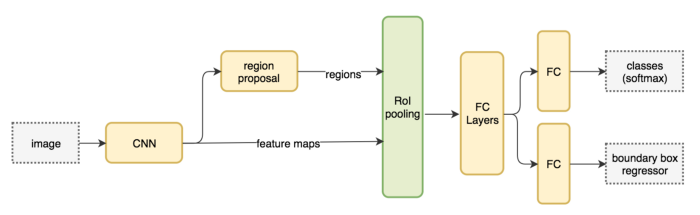
\includegraphics[width=\linewidth]{Sources/Figures/fasterrcnn.png}
    \caption{High-level Faster R-CNN flow. FC stands for fully-connected. \todo{cite}}
    \label{fig:fasterrcnn}
\end{figure}

As we can see, Faster R-CNN firstly computes the feature maps, which are then exploited by two separate computational branches. The region proposal is carried out by a Regional Proposal Network (RPN). The corresponding features of the proposed RoIs are retrieved from the bottom branch's feature maps by a method called RoI pooling. The proposals' feature maps are then fed to the fully-connected network responsible for the final category (class) and bounding box prediction. We describe each component in detail below.

\subsection{Region Proposal Network}
Most of the RPN's architecture looks like a standard CNN image classifier. The network does not predict the raw coordinates, but instead, it learns to predict offsets of reference boxes. We call these reference boxes anchors, and we place them on every point in the feature map (see Figure \ref{fig:rpn}). Each point has several anchors of different sizes and ratios. We predict an "objectness" score for each anchor, which is the anchor's probability of being an object. At the same time, we regress the offsets of the anchors. Since we now have a large set of proposals that can overlap, we apply Non-Maximum Suppression (NMS) to solve the issue of duplicates. NMS is a greedy method that goes through the list of proposals sorted by score and removes proposals with an IoU larger than the predefined threshold with a proposal that has a higher score. Finally, the network outputs top $n$ proposals ($n = 2000$ in original paper).

\begin{figure}[h]
    \centering
    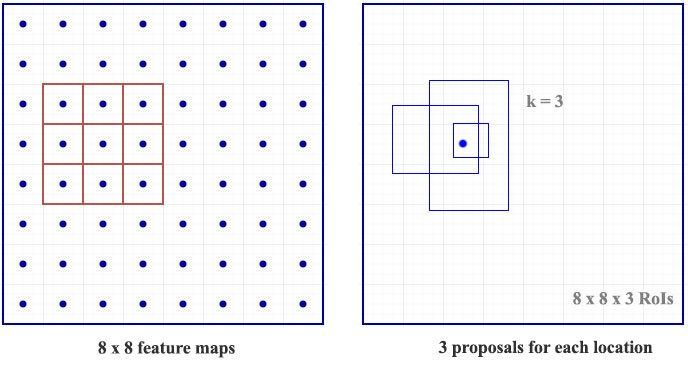
\includegraphics[width=0.7\linewidth]{Sources/Figures/rpn.jpeg}
    \caption{In this illustration, for each point we generate three proposals based on the 3 $\times$ 3 features around the point. \todo{cite}}
    \label{fig:rpn}
\end{figure}

\subsection{RoI Pooling and Fully-connected Layers}
Once we have proposals of different sizes and ratios, we need to convert maps to their corresponding features to fixed-size feature maps because the fully-connected network has a fixed-length input by definition. The conversion is done by RoI pooling layer that takes the input proposals and outputs fixed-size feature maps.  For every input proposal, crop the corresponding section in the input feature map. If we need a $n \times n$ output feature map, we equally divide the section into $n \times n$ blocks. We then apply max-pooling for these blocks, creating a new $n \times n$ feature map. For illustration, see Figure .

\section{Cascade R-CNN}
\section{RetinaNet}

